\section{Results}
\label{sec:results}

\subsection{H1: Bigger models drift less, but the recipe sets the speed}
\label{sec:h1}

\begin{table}[t]
    \centering
    \caption{\pres of general-text probes (final layer) by step. Values are means over seeds; the standard deviation across the three \qwenS seeds is $\leq 0.016$. ``Cross'' is the interpolated step at which preservation first falls below 0.5. ``Health'' compares final with step-0 held-out in-domain NLL. Every run that ends below 0.5 is labelled \emph{diverged}. Highest preservation per column among standard-recipe medical runs in \textbf{bold}.}
    \label{tab:h1}
    \resizebox{\textwidth}{!}{%
    \begin{tabular}{@{}lllccccccll@{}}
        \toprule
        \textbf{Model} & \textbf{Recipe} & \textbf{Domain} & \textbf{10} & \textbf{100} & \textbf{500} & \textbf{1000} & \textbf{2000} & \textbf{3000} & \textbf{Cross} & \textbf{Health} \\
        \midrule
        \pythiaS (2 seeds) & LoRA 2e-4 & medical & 0.89 & 0.57 & 0.42 & 0.46 & 0.36 & 0.31 & $\sim$96--117 & diverged \\
        \pythiaS (2 seeds) & LoRA 2e-4 & code & 0.89 & 0.60 & 0.55 & 0.42 & 0.31 & 0.28 & $\sim$123--224 & diverged \\
        \pythiaS & LoRA 2e-4 & general & 0.89 & 0.46 & 0.39 & 0.40 & 0.45 & 0.43 & $\sim$90 & diverged \\
        \pythiaS & full 1e-5 & medical & 0.90 & 0.83 & 0.79 & 0.70 & 0.65 & 0.62 & never & learned \\
        \pythiaS & full 1e-5 & code & 0.90 & 0.85 & 0.82 & 0.76 & 0.52 & 0.51 & ($\sim$2,240) & no gain \\
        \pythiaM & LoRA 2e-4 & medical & 0.93 & 0.80 & 0.74 & 0.72 & 0.71 & 0.71 & never & learned \\
        \pythiaM & LoRA 2e-4 & code & 0.93 & 0.87 & 0.81 & 0.76 & 0.76 & 0.74 & never & diverged \\
        \midrule
        \qwenS (3 seeds) & LoRA 2e-4 & medical & 0.96 & 0.83 & 0.79 & 0.76 & 0.75 & 0.73 & never & learned \\
        \qwenS (3 seeds) & LoRA 2e-4 & code & 0.98 & 0.91 & 0.87 & 0.84 & 0.82 & 0.81 & never & no gain \\
        \qwenS & LoRA 2e-4 & general & 0.92 & 0.81 & 0.79 & 0.77 & 0.76 & 0.76 & never & learned \\
        \qwenS & LoRA 5e-4 & medical & 0.91 & 0.78 & 0.70 & 0.65 & 0.58 & 0.57 & never & learned \\
        \qwenS & LoRA 5e-4 & code & 0.96 & 0.86 & 0.77 & 0.73 & 0.66 & 0.63 & never & diverged \\
        \qwenS & LoRA 1e-3 & medical & 0.88 & 0.71 & 0.43 & 0.35 & 0.25 & 0.22 & $\sim$420 & diverged \\
        \qwenS & LoRA 1e-3 & code & 0.95 & 0.78 & 0.50 & 0.37 & 0.28 & 0.27 & $\sim$500 & diverged \\
        \qwenM & LoRA 2e-4 & medical & {\bf 0.98} & 0.86 & 0.82 & 0.80 & {\bf 0.78} & (0.77 @2,500) & never & learned \\
        \qwenL & LoRA 2e-4 & medical & {\bf 0.98} & {\bf 0.87} & {\bf 0.85} & {\bf 0.83} & -- & (0.82 @1,500) & never & learned \\
        \bottomrule
    \end{tabular}
    }
\end{table}


\Tabref{tab:h1} and \figref{fig:size_recipe} show \pres of the general-text probes over training.

\para{Scale helps at matched steps.} Within each family, preservation rises with size at every matched step (\figref{fig:size_recipe}, left). After 1,000 medical steps, Qwen preservation is 0.76, 0.80, and 0.83 for 0.5B, 1.5B, and 3B. \pythiaM is far more stable than \pythiaS (0.74 \versus 0.42 at step 500). The direction of H1 therefore holds.

\para{But sub-1B is not enough for collapse.} \qwenS (494M parameters) never falls below 0.71 in 3,000 steps under the standard recipe. Only \pythiaS crosses 0.5 within 500 steps, at roughly steps 90--220.

\para{The learning rate matters more than size.} Raising the LoRA learning rate on \qwenS from 2e-4 to 5e-4 to 1e-3 lowers final medical preservation from 0.73 to 0.57 to 0.22 (\figref{fig:size_recipe}, right). At lr 1e-3, \qwenS crosses 0.5 at steps $\sim$420--500, which matches the H1 prediction. For \pythiaS, full fine-tuning at lr 1e-5 keeps 0.62 after 3,000 medical steps, while LoRA at lr 2e-4 falls to 0.31. A fivefold change in learning rate on one model moves final preservation by 0.51 (0.73 $\rightarrow$ 0.22), while a sixfold change in Qwen size moves step-500 preservation by only 0.06 (0.79 $\rightarrow$ 0.85).

\para{Collapse goes together with failed optimisation.} All seven runs that end below 0.5 have \emph{rising} held-out in-domain NLL. \pythiaS LoRA runs lose 0.5--2.1 nats in every domain, including on \wikitext itself, and \qwenS at lr 1e-3 loses 0.4 (medical) and 1.5 (code) nats. Runs that actually learn their domain end between 0.57 and 0.82. Fast loss of pretraining geometry in these runs is therefore a symptom of destructive optimisation, not of successful specialisation.

\para{Most drift happens early.} In all runs, most of the change happens in the first $\sim$100 steps. After that, curves decline slowly on a log-step axis (\figref{fig:trajectories}).

\para{Fine-tuning itself, not the domain, causes most drift.} The \wikitext control drifts about as much as domain fine-tuning: \qwenS ends at 0.76 after general fine-tuning \versus 0.73 after medical fine-tuning.

\para{Robustness.} $k=5$ and $k=20$ give the same ordering of runs; $k=20$ values are 0.01--0.05 higher. The mean-centred variant is on average 0.024 higher (at most 0.12) with the same ordering. The middle layer is usually somewhat more stable (median $+0.04$) and shows the same pattern.

\begin{figure}[t]
    \centering
    \begin{subfigure}[b]{0.39\textwidth}
        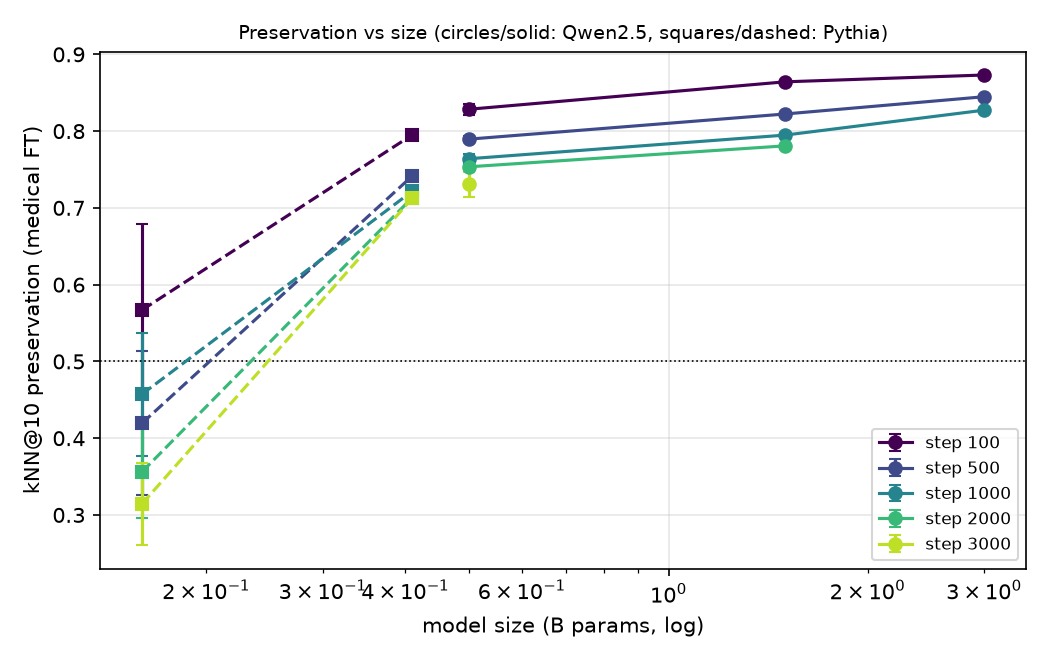
\includegraphics[width=\textwidth]{figures/fig5_preservation_vs_size.png}
        \caption{Preservation \versus model size}
        \label{fig:size}
    \end{subfigure}
    \hfill
    \begin{subfigure}[b]{0.59\textwidth}
        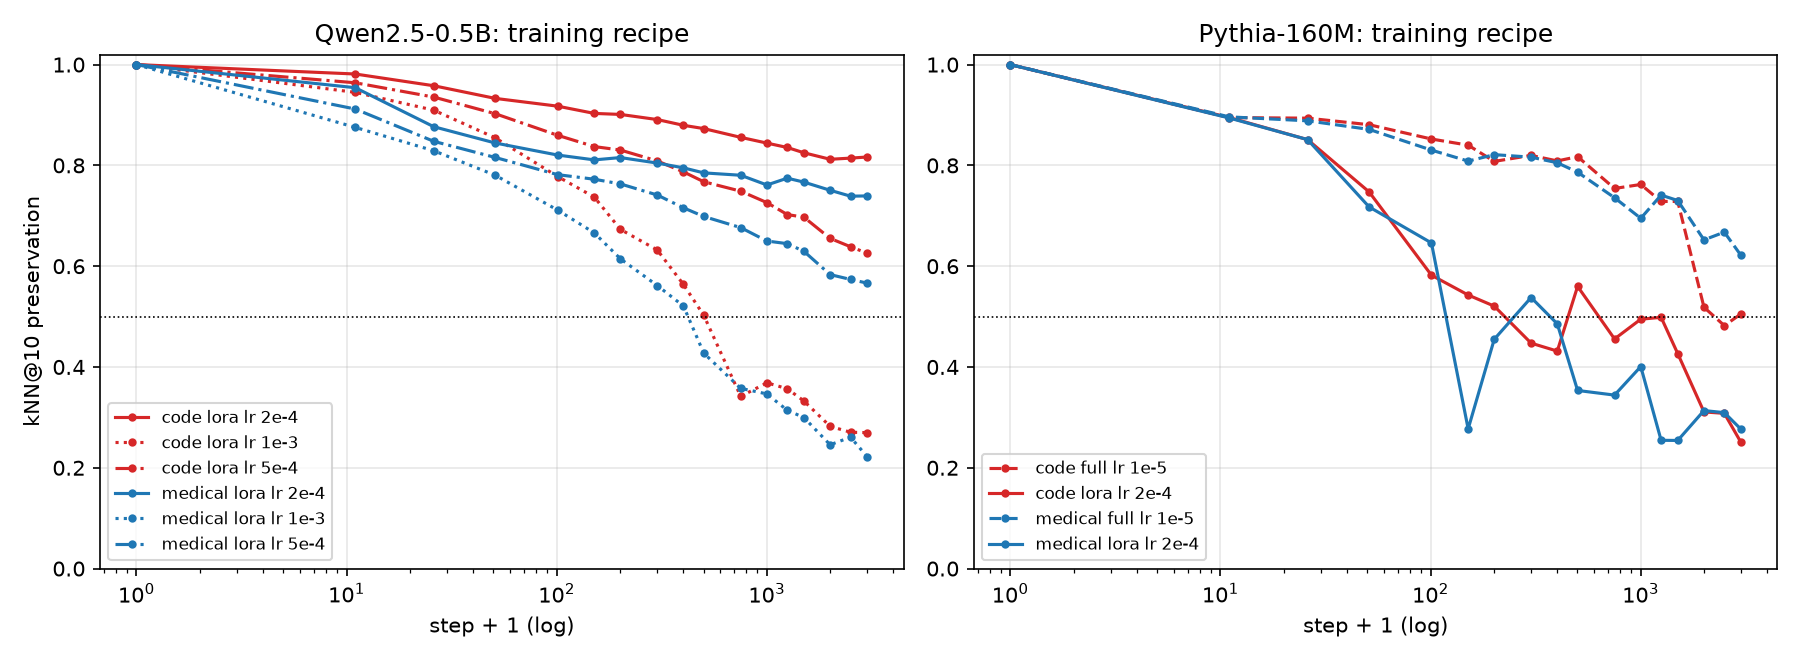
\includegraphics[width=\textwidth]{figures/fig6_recipe_ablation.png}
        \caption{Recipe ablations}
        \label{fig:recipe}
    \end{subfigure}
    \caption{\textbf{(a)} Medical fine-tuning, standard LoRA recipe: preservation grows with size at each step within each family (squares: Pythia; circles: Qwen2.5; error bars over seeds). \textbf{(b)} Changing the recipe on a single model moves preservation much more than size does. For \qwenS, lr 1e-3 drives preservation to $\sim$0.25, and for \pythiaS, full fine-tuning at lr 1e-5 (dashed) drifts far less than LoRA at 2e-4.}
    \label{fig:size_recipe}
\end{figure}

\subsection{H2: Isotropy does not fall monotonically}
\label{sec:h2}

\begin{table}[t]
    \centering
    \small
    \caption{Isotropy change over 22 runs (final layer, general probes). No run moves monotonically toward anisotropy on any measure, and the median net change is a few percent.}
    \label{tab:h2}
    \begin{tabular}{@{}lccc@{}}
        \toprule
        \textbf{Measure} & \textbf{Monotone} & \textbf{Net more anisotropic} & \textbf{Median change} \\
        \midrule
        Mean pairwise cosine ($\uparrow$ anisotropic) & 0 / 22 & 14 / 22 & $+2.3\%$ \\
        \isoscore ($\downarrow$ anisotropic) & 0 / 22 & 18 / 22 & $-8.3\%$ \\
        Effective rank ($\downarrow$ anisotropic) & 0 / 22 & 17 / 22 & $-5.7\%$ \\
        \bottomrule
    \end{tabular}
\end{table}

\Tabref{tab:h2} and \figref{fig:isotropy} summarise isotropy. Most runs end slightly more anisotropic than they started, but none gets there monotonically. \pythiaS LoRA runs first become much \emph{more} isotropic (\isoscore up to 1.6$\times$ its step-0 value at steps 100--500) and then fall back. Meanwhile, local neighbourhood structure loses 20--80\% of its overlap. Fine-tuning reshuffles neighbours long before it changes the global spectral shape of the space. {\bf H2 is not supported}, and global isotropy is a weak drift signal.

\begin{figure}[t]
    \centering
    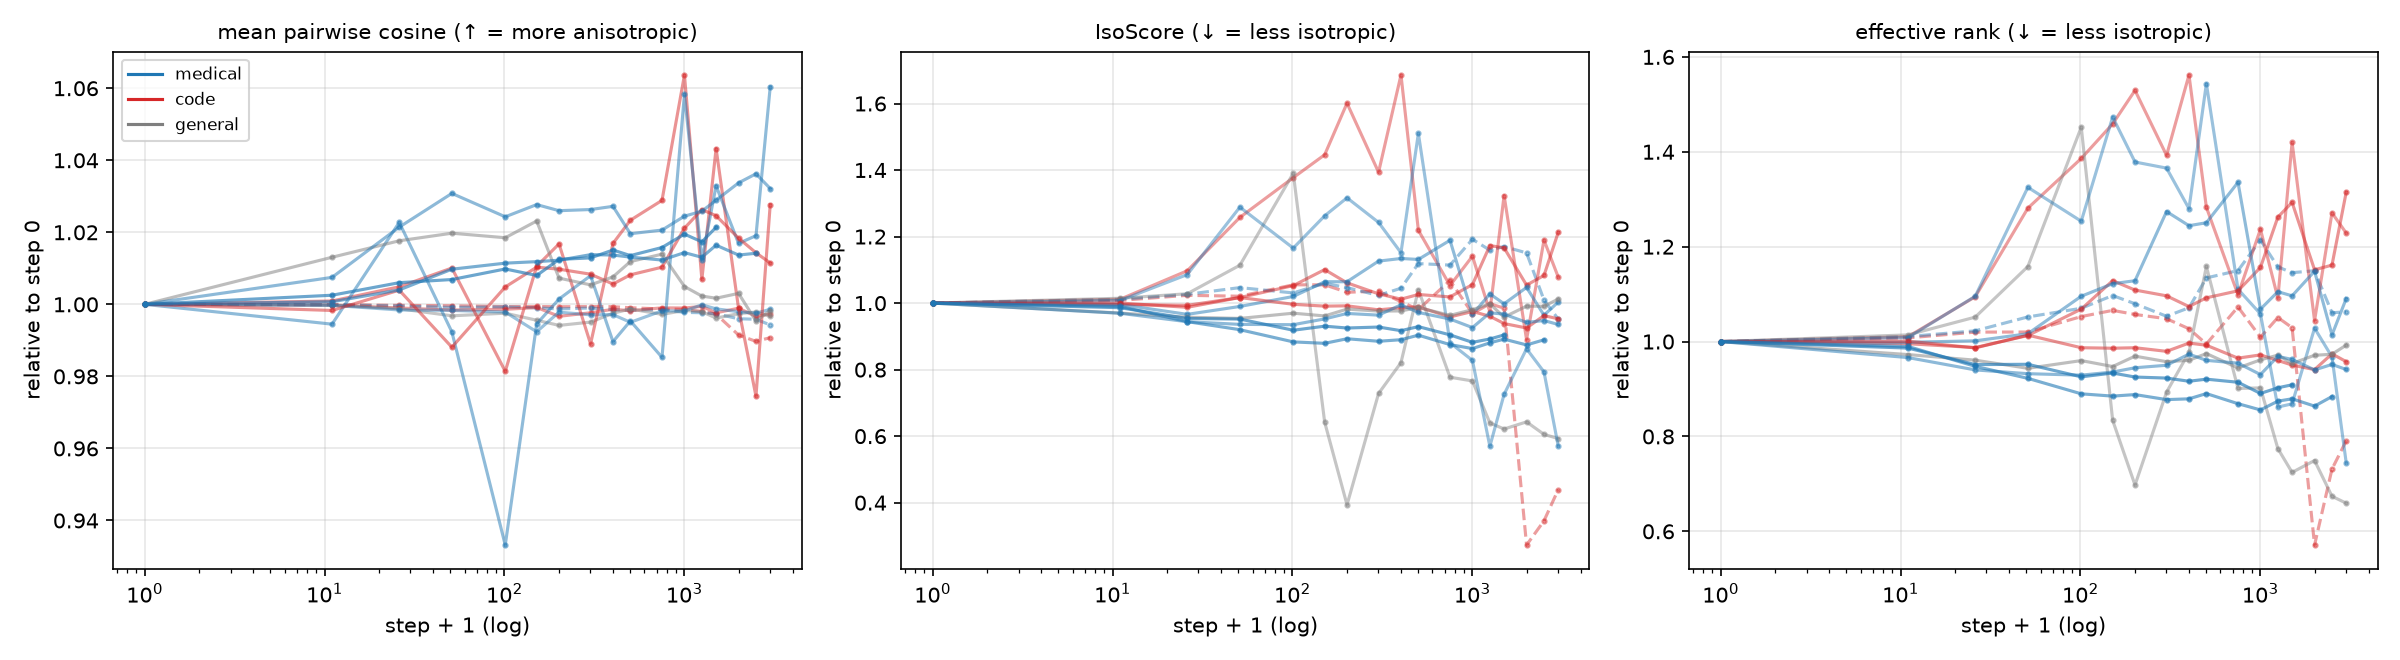
\includegraphics[width=0.95\linewidth]{figures/fig2_isotropy.png}
    \caption{Three isotropy measures relative to step 0 for all runs (blue: medical; red: code; grey: general; dashed: full fine-tuning). Trajectories are noisy and non-monotone, and net changes are small compared with the loss of neighbourhood structure in \figref{fig:trajectories}.}
    \label{fig:isotropy}
\end{figure}

\subsection{H3: Preservation tracks forgetting, but there is no 0.6 threshold}
\label{sec:h3}

\para{Overall association.} Across all 348 non-zero checkpoints, lower preservation goes with more forgetting. Checkpoints with preservation $\geq 0.6$ ($n=260$) lose 2.7\pp \gk accuracy on average, and 39\% show a significant decline. Checkpoints below 0.6 ($n=88$) lose 9.2\pp, and 82\% show a significant decline (Mann--Whitney $p=5\times10^{-12}$). Spearman $\rho$ between preservation and $\Delta$\gk is 0.69, and between preservation and $\Delta$\wikitext NLL it is $-0.90$.

\para{Forgetting starts well above 0.6.} \Tabref{tab:h3_onset} lists the first checkpoint with a significant \gk decline for each run. In 16 of the 21 runs with a detected decline, forgetting begins while preservation is still $\geq 0.6$, usually at 0.77--0.90. \qwenS loses 8.8\pp \gk after 3,000 medical steps and 9.9\pp after 3,000 \wikitext steps, while its preservation stays $\geq 0.71$. At lr 5e-4 it loses 11.7\pp by step 500, at preservation 0.70. The only runs that start forgetting below 0.6 are the diverged \pythiaS LoRA runs.

\begin{table}[t]
    \centering
    \small
    \caption{First checkpoint with a significant drop in general-knowledge accuracy (McNemar $p<.05$ against step 0) and the preservation at that point. Only the \pythiaS LoRA runs, all of which diverged, start forgetting below the hypothesised 0.6 threshold.}
    \label{tab:h3_onset}
    \begin{tabular}{@{}lcc@{}}
        \toprule
        \textbf{Run} & \textbf{Onset step} & \textbf{Preservation at onset} \\
        \midrule
        \qwenS medical (seeds 1/2/3) & 500 / 400 / 750 & 0.79 / 0.80 / 0.77 \\
        \qwenS general & 100 & 0.81 \\
        \qwenS lr 5e-4 (medical / code) & 50 / 300 & 0.82 / 0.81 \\
        \qwenS lr 1e-3 (medical / code) & 50 / 100 & 0.78 / 0.78 \\
        \qwenM medical & 50 & 0.90 \\
        \qwenL medical & 200 & 0.84 \\
        \pythiaM (medical / code) & 150 / 500 & 0.79 / 0.81 \\
        \pythiaS LoRA (5 runs) & 100--300 & 0.43--0.50 \\
        \pythiaS full FT (code / medical) & 1,500 / 2,500 & 0.73 / 0.67 \\
        \bottomrule
    \end{tabular}
\end{table}


\para{The mapping differs across families.} At preservation $\approx 0.25$, \qwenS (lr 1e-3) has lost 30\pp \gk, while \pythiaS has lost only $\sim$4\pp (\figref{fig:forgetting}, left). Part of this gap comes from Pythia's \mmlu accuracy being at chance ($\sim$23\%), so its \gk signal comes only from \arce. Still, the same preservation value means very different amounts of benchmark damage in the two families.

\para{General-text perplexity is the exception.} The relation between preservation and $\Delta$\wikitext NLL is tight and nearly the same for all models (\figref{fig:forgetting}, right). Losing neighbourhood structure on general text goes together with losing general-text language modelling. The one exception is the \wikitext control, where NLL improves while preservation drops. {\bf H3 is not supported}: preservation is associated with forgetting, but there is no onset at 0.6. For Qwen models, accuracy-based forgetting begins around 0.8.

\begin{figure}[t]
    \centering
    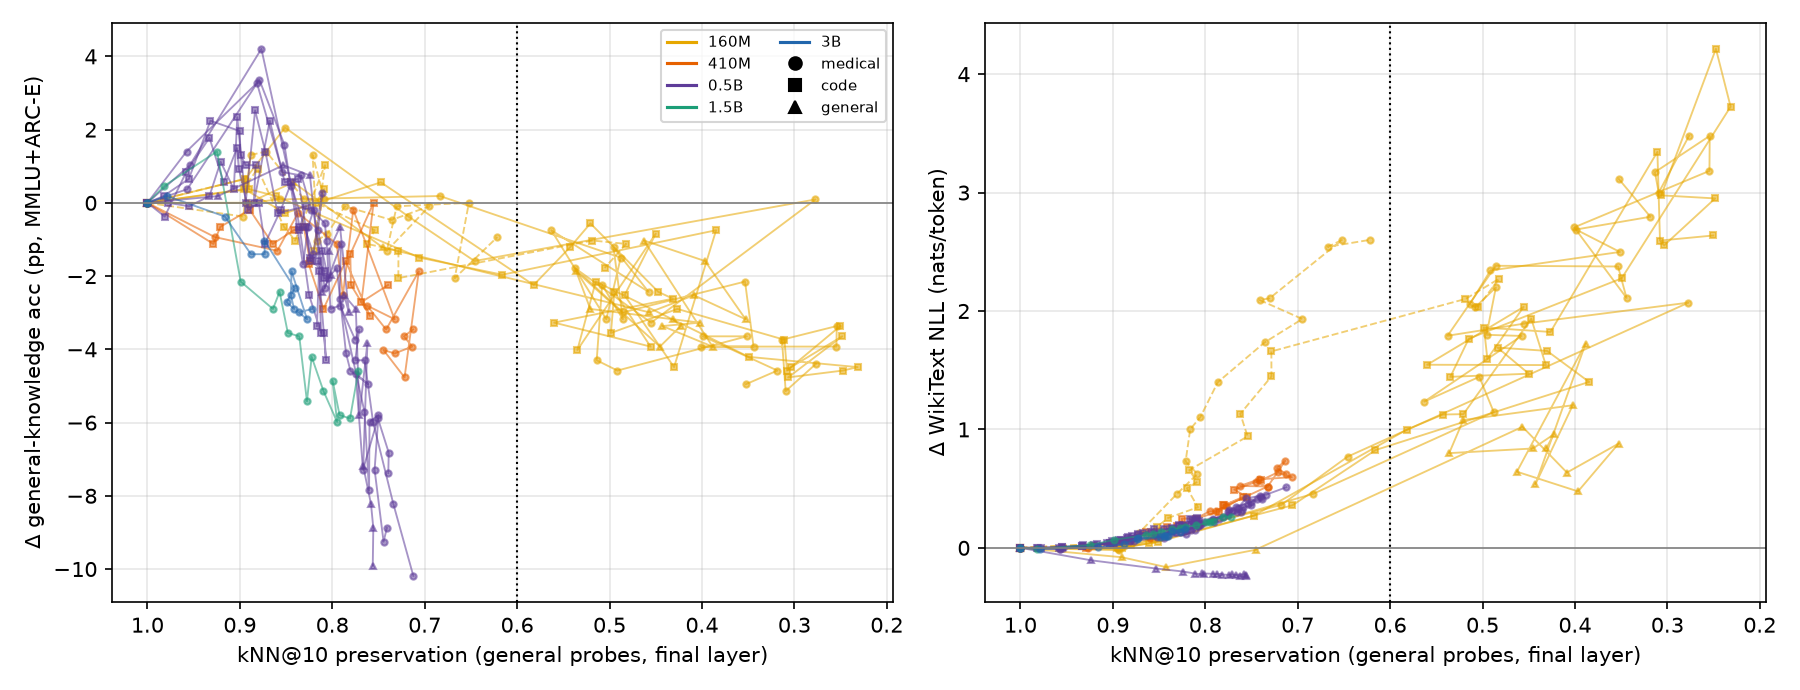
\includegraphics[width=0.95\linewidth]{figures/fig3_preservation_vs_forgetting.png}
    \caption{Preservation against forgetting for every checkpoint (colour: model; marker: domain; dashed: full fine-tuning). \textbf{Left:} change in \gk accuracy. Qwen models (purple, green, blue) lose up to 10\pp while preservation is still above 0.7, whereas \pythiaS (yellow) loses only a few points at 0.3. The dotted line marks the hypothesised 0.6 threshold. \textbf{Right:} change in \wikitext NLL. The relation is tight and shared across models; the lower branch is the \wikitext control run.}
    \label{fig:forgetting}
\end{figure}

\subsection{H4: Code preserves more general geometry than medical text}
\label{sec:h4}

\begin{table}[t]
    \centering
    \small
    \caption{Medical \versus code fine-tuning. \textbf{Top:} paired differences over 144 checkpoints matched on model, recipe, seed, and step (Wilcoxon signed-rank). Negative preservation differences mean medical preserves \emph{less}. \textbf{Bottom:} vocabulary overlap of each corpus with \wikitext ($\sim$2M Qwen tokens each). Medical text is much closer to general text, yet it preserves less general-text geometry.}
    \label{tab:h4}
    \begin{tabular}{@{}lcc@{}}
        \toprule
        \textbf{Paired comparison} & \textbf{Medical $-$ code} & \textbf{$p$} \\
        \midrule
        \pres & $-0.043$ (medical higher at 17\%) & $3\times10^{-12}$ \\
        Centred \pres & $-0.044$ & $3\times10^{-14}$ \\
        CKA & $-0.011$ & $2\times10^{-11}$ \\
        $\Delta$ \gk accuracy & $-1.9$\pp (medical forgets more) & $3\times10^{-10}$ \\
        $\Delta$ \wikitext NLL & $+0.21$ nats (medical forgets more) & $9\times10^{-18}$ \\
        \midrule
        \textbf{Corpus overlap with \wikitext} & \textbf{Medical} & \textbf{Code} \\
        \midrule
        Unigram JSD (bits, $\downarrow$ closer) & {\bf 0.45} & 0.63 \\
        Token mass in top-10k \wikitext tokens & {\bf 67\%} & 36\% \\
        Word-type coverage & {\bf 90\%} & 80\% \\
        \bottomrule
    \end{tabular}
\end{table}


\para{The premise holds; the prediction fails.} Clinical notes are much closer to \wikitext than Python code is (JSD 0.45 \versus 0.63 bits; \tabref{tab:h4}). Yet over 144 matched checkpoints, medical fine-tuning preserves \emph{less} general-text geometry than code ($-0.043$, medical higher at only 17\% of checkpoints, $p=3\times10^{-12}$). Medical fine-tuning also causes more forgetting: 1.9\pp more \gk loss and 0.21 nats more \wikitext NLL increase. All three \qwenS seeds agree (final preservation 0.74 / 0.71 / 0.74 for medical \versus 0.82 / 0.81 / 0.81 for code), as do \qwenS at lr 5e-4 (0.57 \versus 0.63) and 1e-3 (0.22 \versus 0.27), and \pythiaM (0.71 \versus 0.74). Only \pythiaS follows H4's direction (LoRA: 0.28 / 0.35 \versus 0.25 / 0.30; full fine-tuning: 0.62 \versus 0.51), and its LoRA runs diverged in both domains.

\para{Two possible explanations.} The first is \emph{interference}. Clinical English uses the same tokens and features as general English, so adapting to it rewrites features that general text depends on, while code lives in a more separate region of the space. The second is \emph{amount of change}. The base models already model this Python corpus well. Under the standard recipe, code fine-tuning gave no in-domain gain for \qwenS (held-out NLL 1.58 $\rightarrow$ 1.68), while medical fine-tuning really adapted the model (2.34 $\rightarrow$ 1.98). Small, noise-like updates should move the geometry less. Our design cannot separate these two explanations, because the domain contrast is confounded with how much there is to learn. Either way, {\bf H4 is not supported}, and vocabulary overlap does not predict geometric preservation here. As expected for real domain adaptation, under medical fine-tuning the medical probes move the most (\qwenS: 0.64 for medical probes \versus 0.74 for general probes).
